%% LyX 2.1.2 created this file.  For more info, see http://www.lyx.org/.
%% Do not edit unless you really know what you are doing.
\documentclass[english]{paper}
\usepackage[T1]{fontenc}
\usepackage[utf8]{luainputenc}
\usepackage{geometry}
\geometry{verbose,bmargin=2cm}
\setcounter{secnumdepth}{2}
\setcounter{tocdepth}{2}
\usepackage{float}
\usepackage{calc}
\usepackage{graphicx}

\makeatletter

%%%%%%%%%%%%%%%%%%%%%%%%%%%%%% LyX specific LaTeX commands.
%% Because html converters don't know tabularnewline
\providecommand{\tabularnewline}{\\}

%%%%%%%%%%%%%%%%%%%%%%%%%%%%%% User specified LaTeX commands.
\usepackage{graphics}
\usepackage{graphicx}

\makeatother

\usepackage{babel}
\begin{document}

\title{Advanced Systems Lab}


\subtitle{Milestone 1 Report}


\author{Karolos Antoniadis}

\maketitle
This is the report of the first milestone of ``Advanced System Lab''
project. The report starts with an introduction of the system created
for this milestone. Afterwards, in Section \ref{sec:systemdesign}
we describe the general design of the system, including the database,
the middleware and the clients. In Section \ref{sec:testing} we describe
how we tested the system. We follow with a description of the experimental
setup and how the experiments were conducted in Section \ref{sec:experimentalsetup}.
In Section \ref{sec:experiments} we continue by describing the experiments
that were done and their evaluation. We conclude the report in Section
\ref{sec:conclusion}.


\section{Introduction\label{sec:introduction}}

Goal of this milestone was to create a message passing system supporting
persistent queues and a simple message format. Furthermore to experimentally
evaluate it and determine its performance characteristics. The desired
message passing system consists of three tiers. The first one implements
the persistent queues using a database, which from now on will be
referred as the ``database tier'' or ``database'' (db). The second
tier implements the messaging system and is responsible of all the
logic related to system management, also it is the one tier that is
using the database in order to implement its functionality. We will
refer to this tier as the ``middleware tier'' or ``middleware''
(mw). Finally, the third tier that implements the clients that send
and receive messages using the middleware, this tier is going to be
referred to as ``clients tier'' or simply ``clients''. Figure
\ref{tiers} depicts the three tiers and they way they are connected
to each other. As can been seen in the figure there is only one database
while there can be more than one middlewares that are identical to
each other and are connected to the database, as well as many clients
connecting to different middlewares. 

\begin{figure}[H]
\begin{centering}
\includegraphics[scale=0.25]{images/tiers}
\par\end{centering}

\protect\caption{The Three Tiers}
\label{tiers}
\end{figure}



\section{System Design and Implementation\label{sec:systemdesign}}

In this section we describe the design of our system. We start by
describing the code structure of our implementation and its main interface
and aftewards we look more thoroughly at every tier and how its functionality
was implemented.


\subsection*{Code Structure and Interfaces Overview}

All the code for the client and the middleware was implemented in
subpackages of \textit{ch.ethz.inf.asl}. The package structure can
be seen in Figure \ref{packages}.

\begin{figure}[H]
\fbox{\begin{minipage}[t]{1\columnwidth}%
ch.ethz.inf.asl

\fbox{\begin{minipage}[t]{0.99\textwidth}%
client :: contains classes related to client code

common :: package containing common classes to be used by both the
clients and the middleware

\fbox{\begin{minipage}[t]{0.99\textwidth}%
request :: contains all the possible request classes and the \textit{Request}
abstract class

response :: contains all the possible response classes and the\textit{
Response} abstract class%
\end{minipage}}

console :: containts the management console code

exceptions :: contains relevant exceptions used by the application

logger :: contains the \textit{Logger} class used for instrumenting
the system

main :: contains the Main class that is used to start the clients
and the middleware

middleware :: package containing classes related to the middleware

\fbox{\begin{minipage}[t]{0.99\textwidth}%
pool :: package containing pool implementations

\fbox{\begin{minipage}[t]{0.99\textwidth}%
connection :: contains the implementation of a connection pool

thread :: contains the implementation of a thread pool%
\end{minipage}}%
\end{minipage}}

utils :: contains general utility methods for the application%
\end{minipage}}%
\end{minipage}}



\protect\caption{Package Structure}
\label{packages}

\end{figure}


While designing the system we came to the realization that the communication
protocol, meaning the messages that are being sent, for example send
message, receive message etc. are the same between the clients and
the middleware and bewteen the middleware and the database. They are
the same in the sense that when a client wants to send a message he
has to issue some kind of send message request to the middleware.
Similarly when the middleware wants to serve a send message request
or the client he can issue a send message to the database. Because
of this we created the interface that can be seen in Figure \ref{protocol}.
This interface can be found in the \textit{MessagingProtocol} interface
and is implemented by both \textit{ClientMessagingProtocolImpl} and
\textit{MiddlewareMessagingProtocolImpl} classes. The difference between
the two implementations is that in the client implementation when
for example \textit{sendMessage(...)} is called an underlying connection
is used to a send a message from the client to the middleware that
informs the middleware of the desire of the client to send a message.
While on the other hand when the middleware calls \textit{sendMessage(...)}
the middleware is calling a stored function from the database to actually
``save'' the message in the database. More on how this interface
waas implemented by the client and the middleware is given in their
corresponding subsections.

\begin{figure}[H]
\fbox{\begin{minipage}[t]{1\columnwidth}%
\textit{int sayHello(String clientName);}

\textit{void sayGoodbye();}

\textit{int createQueue(String queueName);}

\textit{void deleteQueue(int queueId);\\}

\textit{void sendMessage(int queueId, String content);}

\textit{void sendMessage(int receiverId, int queueId, String content);}

\textit{Optional<Message> receiveMessage(int queueId, boolean retrieveByArrivalTime);}

\textit{Optional<Message> receiveMessage(int senderId, int queueId,
boolean retrieveByArrivalTime);}

\textit{Optional<Message> readMessage(int queueId, boolean retrieveByArrivalTime);}

\textit{int{[}{]} listQueues();}%
\end{minipage}}

\protect\caption{Messaging Protocol Interface}
\label{protocol}
\end{figure}


As can be seen from Figure \ref{protocol} the retrieving messages
methods use the \textit{retrieveByArrivalTime} parameter. If this
parameter is true then the message retrieved is the oldest one. The
\textit{readMessage()} method is different to its corresponding \textit{receiveMessage()}
method since it only reads a message from the system but is not actually
removing it. 


\subsection*{Database}

The PostgreSQL database management system was used, specifically PostgreSQL
(release 9.3.5). It was need for the system to persistent store information
so a database was used to store the needed information for the clients,
the queues and the messages. For this reason three tables were created
as can been seen in Figure \ref{tables} with their fields and their
respective SQL types. As can been seen in this figure the fields \textit{sender\_id},\textit{
receiver\_id }and\textit{ queue\_id }are all foreign keys of the\textit{
message }table. The first two are associated with the\textit{ id }of
the \textit{client }table, while\textit{ queue\_id} is connected to
the\textit{ id }of the\textit{ queue }table.

\begin{figure}[H]
\begin{centering}
\textit{}%
\begin{tabular}{|c|}
\hline 
\textit{client}\tabularnewline
\hline 
\hline 
\textbf{\textit{id}}\textit{ serial primary key}\tabularnewline
\hline 
\textbf{\textit{name }}\textit{varchar(20) NOT NULL}\tabularnewline
\hline 
\end{tabular}\textit{\hspace{0.5cm}}%
\begin{tabular}{|c|}
\hline 
\textit{queue}\tabularnewline
\hline 
\hline 
\textbf{\textit{id}}\textit{ serial primary key}\tabularnewline
\hline 
\textbf{\textit{name}}\textit{ varchar(20) NOT NULL}\tabularnewline
\hline 
\end{tabular}
\par\end{centering}

\vspace{0.5cm}

\begin{centering}
\textit{}%
\begin{tabular}{|c|}
\hline 
\textit{message}\tabularnewline
\hline 
\hline 
\textbf{\textit{id}}\textit{ serial primary key}\tabularnewline
\hline 
\textbf{\textit{sender\_id}}\textit{ integer REFERENCES client(}\textbf{\textit{id}}\textit{)
NOT NULL}\tabularnewline
\hline 
\textbf{\textit{receiver\_id}}\textit{ integer REFERENCES client(}\textbf{\textit{id}}\textit{)}\tabularnewline
\hline 
\textbf{\textit{queue\_id}}\textit{ integer REFERENCES queue(}\textbf{\textit{id}}\textit{)
NOT NULL}\tabularnewline
\hline 
\textbf{\textit{arrival\_time}}\textit{ timestamp NOT NULL}\tabularnewline
\hline 
\textbf{\textit{message}}\textit{ text NOT NULL}\tabularnewline
\hline 
\end{tabular}
\par\end{centering}

\protect\caption{Tables\label{tables}}
\end{figure}


As can be seen all of the fields except the \textit{receiver\_id}
of the \textit{message} table cannot contain the \textit{NULL} value.
This was a deliberate choice since it is possible for a message to
be sent with no particular receiver in mind and such a message could
possibly be received by any other client (except the client that sent
the message). In such a case, i.e. a message has no specific receiver,
the \textit{receiver\_id }contains the \textit{NULL} value.

The \textit{message} table has also two check constraints associated
with it. Those constraints are: 
\begin{enumerate}
\item \textit{CONSTRAINT check\_length CHECK (LENGTH(message) <= 2000)}
\item \textit{CONSTRAINT check\_cannot\_send\_to\_itself CHECK (sender\_id
!= receiver\_id)}
\end{enumerate}
The \textit{check\_length} constraint checks that a message cannot
contain a message with too much content, in this case one with more
than 2000 characters, this constraint was removed during the ``increasing
message size'' experiment. The second constraint was added because
it was considered meaningless for a client to send a message to himself.
It is also considered meaningless for a client to receive a message
he sent (in case the \textit{receiver\_id} is \textit{NULL}), this
is also checked in the stored function and is explained later on.

In order to increase the performance of the database, indexes were
used. PostgreSQL creates by default indexes on the primary keys%
\footnote{``Adding a primary key will automatically create a unique btree index
on the column or group of columns used in the primary key.'' (http://www.postgresql.org/docs/9.3/static/ddl-constraints.html)%
}. The extra indexes that were introduced are the following: 
\begin{enumerate}
\item \textit{CREATE INDEX ON message (receiver\_id, queue\_id)}
\item \textit{CREATE INDEX ON message (sender\_id)}
\item \textit{CREATE INDEX ON message (arrival\_time)}
\end{enumerate}
The first index was introduced to make faster the retrieval of message
since most of them are based on a \textit{receiver\_id }and on a \textit{queue\_id}.
Note that the field \textit{receiver\_id} appears first on this multicolumn
index, this was not a random choice since it is known%
\footnote{``...but the index is most efficient when there are constraints on
the leading (leftmost) columns.'' (http://www.postgresql.org/docs/9.3/static/indexes-multicolumn.html)%
} that the in a multicolumn index the leftmost column can also be efficiently
used solo. The case where \textit{receiver\_id} is used alone and
not in combination with \textit{queue\_id} is the listing queues query
that lists the queues where a message for a client exists. The second
index was created to speed up receiving of messages from a specific
sender. The third index was introduced since some of the receiving
messages functions receive messages based on the arrrival time. 

Code for the creation of the tables and the indexes can be found in
the \texttt{auxiliary\_functions.sql} file in \texttt{src/main/resources}.


\subsubsection*{Stored Functions}

Stored functions were created using the PL/pgSQL procedural language
to reduce the network communication time between the middleware and
the database. Also stored functions have the advantage that they are
compiled already by the DBMS and their query plan has been generated
so they can be reused and therefore increa\emph{se} performance. The
code for the stored functions can be found in \texttt{read\_committed\_basic\_functions.sql}
file in \texttt{src/main/resources} and all of them are used to be
able to implement the interface shown in Figure \ref{protocol}.

The stored functions \textit{read\_message} and \textit{receive\_message}
specifically check that if a message has no receiver it is not being
returned to the client that sent it since this cannot be catched by
the \textit{check\_cannot\_send\_to\_itself} constraint because in
those cases the \textit{receiver\_id} is \textit{NULL}.

Stored functions were not used everywhere, only where it made sense.
For example in cases where the same SQL queries did not need to be
executed many times, simple queries were sent to the database instead,
e.g. management console.


\subsubsection*{Transactions and Isolation Levels}

In this subsection we discuss isolation levels and why they are important
for the correctness of our system. In order to do so let us see a
simplified version of the internals of the \textit{receive\_message}
stored function, seen in Figure \ref{receiveMessage}, that takes
two parameters, the \textit{p\_requesting\_user\_id} and the \textit{p\_queue\_id}
and is trying to find a message for the requesting user in the given
queue.
\begin{figure}[H]
\centering{}\textit{}%
\fbox{\begin{minipage}[t]{1\columnwidth}%
\textit{SELECT id INTO received\_message\_id FROM message WHERE queue\_id
= p\_queue\_id AND receiver\_id = p\_requesting\_user\_id LIMIT 1;}

\textit{RETURN QUERY SELECT {*} FROM message WHERE id = received\_message\_id;}

\textit{DELETE FROM message where id = received\_message\_id; }%
\end{minipage}}\protect\caption{Simplified Version of \textit{receive\_message} Body }
\label{receiveMessage}
\end{figure}


Functions in PostgreSQL are executed within transactions%
\footnote{``Functions and trigger procedures are always executed within a transaction
established by an outer query'' (http://www.postgresql.org/docs/current/interactive/plpgsql-structure.html)%
}. Transactions are known to be atomic, in the sense that they either
``happen'' completely, i.e. all their effects take place, or not
at all. But still problems could arise! The default isolation level
in PostgreSQL is READ COMMITTED%
\footnote{http://www.postgresql.org/docs/9.3/static/transaction-iso.html\label{fn:transactionsLink}%
} which roughly states ``...a SELECT query (without a FOR UPDATE/SHARE
clause) sees only data committed before the query began; it never
sees either uncommitted data or changes committed during query execution
by concurrent transactions.''\textsuperscript{\ref{fn:transactionsLink}}.
So with such an isolation level it is possible for two concurrent
transactions to read the exact same message, only one of them will
delete it, but both of them will return it. This of course is not
acceptable since we want a message to be read by only one client.
In order to solve this problem there are at least two approaches:
\begin{enumerate}
\item Use \textit{FOR UPDATE}%
\footnote{``FOR UPDATE causes the rows retrieved by the SELECT statement to
be locked as though for update. This prevents them from being modified
or deleted by other transactions until the current transaction ends.``
and ``That is, other transactions that attempt UPDATE, DELETE, SELECT
FOR UPDATE, SELECT FOR NO KEY UPDATE, SELECT FOR SHARE or SELECT FOR
KEY SHARE of these rows will be blocked until the current transaction
ends. `` (http://www.postgresql.org/docs/9.3/static/sql-select.html\#SQL-FOR-UPDATE-SHARE)\label{fn:FOR-UPDATE-causes}%
}and therefore prevent other transactions from selecting the same message.
\item Change isolation level to \textit{REPEATABLE READ} which is stronger
than \textit{READ COMMITTED} and roughly states  ``This level is
different from Read Committed in that a query in a repeatable read
transaction sees a snapshot as of the start of the transaction, not
as of the start of the current query within the transaction.''\textsuperscript{\ref{fn:transactionsLink}}.
In case another transaction deletes the message in the meantime the
transactions is going to fail by giving back an error. 
\end{enumerate}
The ``problem'' with the second approach is that a transaction could
find concurrent update errors and will have to be re-executed: ``...it
should abort the current transaction and retry the whole transaction
from the beginning.''\textsuperscript{\ref{fn:transactionsLink}}.
For the above reasons we used the first approach since it made our
application code easier, i.e. not having to repeat a transaction.

We have to mention here that the \textit{SELECT} command combined
with \textit{FOR UPDATE} and \textit{ORDER BY} could have some problems:
``It is possible for a SELECT command running at the READ COMMITTED
transaction isolation level and using \textit{ORDER BY} and a locking
clause to return rows out of order.''\textsuperscript{\ref{fn:FOR-UPDATE-causes}}.
This is because ordering of the rows occurs before locking them, so
it is possible that when the rows are locked some columns might have
been modified. This is not a problem in our implementation since we
delete the selected row.


\subsubsection*{Connecting Java and PostgreSQL}

For the connection between Java and the database the JDBC41 PostgreSQL
driver%
\footnote{http://jdbc.postgresql.org/download.html%
} was used.


\subsubsection*{What is being logged?}

The only thingthat is being logged in the database while it is being
used is he the CPU, network and memory utilization using the dstat%
\footnote{http://dag.wiee.rs/home-made/dstat/%
} tool.


\subsubsection*{Management Console}

A management console was also created (it is implemented in the \textit{Manager}
class under the \textit{console} package) to easily check the contents
of a database in a remote machine. The console is a GUI application
and can be seen Figure \ref{management}. The user of the console
just has to provide the host address and port number of where the
database is running, as well as the username, password and database
name. Then by clicking ``Login'' and the appropriate ``Refresh''
buttons he can check the current data of the client, queue or message
table. For retrieving the data from the database simple ''\textit{SELECT
{*} FROM ...}`` queries were issued on the database, no stored functions
were created for this since they are only used for the console and
quite sparingly.

\begin{figure}[H]
\begin{centering}
\includegraphics[scale=0.4]{images/management}\protect\caption{Management Console Screenshot}
\label{management}
\par\end{centering}

\end{figure}


In order to use the management console the \textit{main()} method
from the\textit{ Manager} class needs to be executed.


\subsection*{Middleware}

The middleware implements the messaging system, it receives requests/messages
from clients and has to use the database in order to persist those
messagess, as well as retrieve the messages from the database to return
to the clients. Obviously if we want to be able to support more than
one client the middleware needs to be multi-threaded. The interface
that the middleware has to implement can be seen in Figure \ref{protocol}.

Our middleware follows a non-blocking approach using simple Java IO.
This seems hard to believe at first but nevertheless this is the case
as will be explained later on. But before doing so, let us see some
of the possible approaches that can be used to implement a middleware.
\begin{itemize}
\item In this approach the middleware would have some threads, also known
as worker threads, on the middleware and every one of them waits for
a connection from the client. When a connection is established the
thread blocks and waits for a request from the client. When it receives
the request it, it executes the request meaning it issues the corresponding
operations to the database and then returns the response back to the
client. Afterwards it closes the connection and waits for the next
client connection. Although this approach can support an arbitrary
number of client it is quite wasteful and slow since for every request-response
interaction the client has to establish a connection with the middleware. 
\item With this approach we have a worker thread for every client. A worker
thread is created when a client connects and then it is used for this
client until the end. The advantage of this approach in constrast
to the previous is that there does not have to be an establishment
of a connection for every request between the client and the middleware.
But this solution seems to have scalability issues since the number
of clients the middleware could possibly support is bounded by the
number of threads the system can support. 
\item This approach uses Java New IO. The rough idea is having a thread,
called selector thread, that blocks until a new connection from a
clien is established or data from some already established connection
are received. When data from a connection are received the reading
of the data can be passed to a worker thread that is going to do the
actual reading and the one that is going to send the response back
to the client. This solution has none of the above problems.
\end{itemize}
Our approach followed a different way. Its main idea is to have a
queue of sockets corresponding to connections from the clients. Everytime
a client connects to the middleware the socket is being added to this
queue. Then there are also some worker threads operating in a round-robin
approach on this queue and check if there is something to read from
the underlying input stream of the socket. If yes they read the data,
use the database to perform their operation and send the response
back to the client. This approach has none of the problems described
in the first two approaches. Our implementation of this approach is
non-blocking since a worker thread never blocks to wait for data from
a specific connection, if there are no data in a connection it just
puts the connection back to the queue and continues with the next
connection. The non-blocking implemenation was achieved by using \textit{InputStream}'s
\textit{available()} method that can return the number of bytes that
can be read whithout blocking. \textit{available()} is of course a
non-blocking method which means a worker thread issues a blocking
\textit{read()} method call only when \textit{available()} showed
that a number of bytes can be read without blocking. In Figure \ref{middlewareArchitecture}
the architecture of our middleware is depicted while in Figure \ref{workerThread}
it is shown how a middleware's worker thread operates.

\begin{figure}[H]


\centering{}\includegraphics[scale=0.21]{images/middlewareArchitecture}\protect\caption{Middleware Architecture}
\label{middlewareArchitecture}
\end{figure}


As can be seen in Figure \ref{middlewareArchitecture} the worker
threads of the middleware interact with the sockets queue, as well
as with the connection pool in order to get a connection to the database
for issuing their request. Note furthermore that the ``waiting for
a connection'' part of the middleware is blocking.

\begin{figure}[H]
\begin{centering}
\includegraphics[scale=0.22]{images/workerThread}
\par\end{centering}

\protect\caption{Worker Thread of the Middleware}
\label{workerThread}

\end{figure}



\subsubsection*{Middleware Implementation}

The implementation of the middleware is located under the package
with the same name: \textit{ch.ethz.inf.asl.middleware}. This package
contains the following classes:
\begin{itemize}
\item \textit{Middleware}: this is the class that needs to be instantiated
to start the middleware. It is constructed using a configuration,
what is needed for the configuration is explained later on. By calling
its \textit{start()} method the middleware initializes the thread
pool and waits for upcoming connections from clients. When a client
connects his corresponding connection is inserted into the sockets
queue.
\item \textit{MiddlewareRunnable}: this class corresponds to a worker thread.
It is being constructed with the middleware's sockets queue as well
as the connection pool created from the middleware.
\item \textbf{\textit{InternalSocket}}: the middleware socket queue does
not actually contain immediate\textit{ Socket (javat.net.Socket)}
objects but actually \textit{InternalSocket} objects. An internal
socket contains internally a normal Java socket as well as some extra
methods. For instance it has a method that returns the last time this
socket was worked on (\textit{getLastTime()}), this method is helpful
for logging purposes, i.e. we can now know how much a socket was waiting
on the sockets queue before it was picked by a worker thread. This
class also supports reading data in chunks! Because we use the \textit{available()}
method as was said previously it is possible to have only 1 byte available
per time and in such cases we need somehow to accumulate the read
bytes until we have read the full request. \textit{InternalSocket}
achieves this operation by calling \textit{addData(byte{[}{]} readData)}
every time we read some bytes and we can get the accumulated bytes
until now by calling \textit{getObjectData()}.
\item \textit{MiddlewareMessagingProtocolImpl}: this class implements the
\textit{MessagingProtocol} interface and is the one that actually
calls the stored functions.
\end{itemize}

\subsubsection*{Thread \& Connection Pool}

Our own thread and connection pools were implemented, their code can
be found under the \textit{ch.ethz.inf.asl.middleware.pool.thread}
and \textit{ch.ethz.inf.asl.middleware.pool.connection} packages in
the \textit{ThreadPool} and \textit{ConnectionPool} classes respectively.
Let us see each of these classes:
\begin{itemize}
\item \textit{ThreadPool}: this class is instatiated given the number of
threads the desired pool needs to have. This class creates the given
amount of threads and executes them, every one of those threads waits
to receive another thread submitted by the user of the thread pool
to execute it. In order to execute a thread we just have to call the
pool's \textit{execute(Runnable command)} method that just adds the
\textit{command} in the queue to be executed. The \textit{execute()}
method might block if the underlying queue is full. The queue of the
threads that is used internally by this classes to ``save'' the
commands is a Java's \textit{ArrayBlockingQueue} queue, that is, a
thread-safe bounded queue implemenation that orders elements \textbf{FIFO}
(first-in-first-out).
\item \textit{ConnectionPool}: this class can be constructed given the maximum
amount of connections we need and the login credentials of the database.
Afterwards a call to \textit{getConnection()} returns a \textit{Connection}
object. Until the maximum number of connections is reached, new connections
are being created on every call to \textit{getConnection()}, afterwards
they are being re-used. The \textit{getConnection()} method blocks
when there are no more available connections at the moment. When the
\textit{close()} method is called on a \textit{Connection} object
returned by \textit{getConnection()} the closed connection is not
actually closed but just returned back to the pool to be re-used.
This was achieved by creating the \textit{InternalConnection} inner
class tha contains a Java's \textit{Connection} object internally
and also extends the \textit{Connection} class. Whenever a call to
an \textit{InternalConnection} method is issued the corresponding
\textit{Connection} object method is called. Except in the case when
the \textit{close()} method is called in which case the specific connection
is returned back to the pool. The connection pool can also be closed
by calling its respective \textit{close() }method which is going to
close all the connections currently existing in the pool, or it can
be used in a try-with-resources statement since it implements the
\textit{AutoCloseable} interface. Internally the connection pool uses
\textit{ArrayBlockingQueue} similarly to the thread pool implementation.
This means that requests to \textit{getConnection()} that are waiting
are waiting in a FIFO way.
\end{itemize}

\subsubsection*{Serialization of Messages}

A question that might arise by reading this report until now might
be how are requests and responses formatted before being transmitted
between the clients and the middleware. Answer: they are serialized.
All the requests and all the responses implement the \textit{Serializable}
interface, so they can easily be serialized to a \textit{byte} array.
This array's length is calculated and the resulted length is transformed
to exactly 4 bytes (1 \textit{int}). The length is concatenated with
the serialized byte array, with the length being in the front. This
concatanted array is what is being transmitted between the client
and the middleware. The length is added so when the middleware starts
reading data from the client it can read the length of the upcoming
object (look \textit{InternalSocket}) and know when to stop reading.
When it reads the whole data, it removes the length part and deserializes
the remaining byte array to get the \textit{Request} object. The middleware
creates the response in the exact same way before sending it to the
client. Although this is not necessary for the client, since the client
blocks until he reads the response. But it was done nevertheless for
consistency reasons so the clients and the middlewares send and receive
in the same way.


\subsubsection*{Where do requests get queued up?}

From the above description of the system it is easy to see that there
are two main parts of the system were a request could stuck waiting.
The one is in the sockets queue waiting until its socket is being
worked on by a worker thread. The second part is waiting for the connection,
after getting the request the middleware might have to wait for others
worker threads to finish their database requests until it is able
to proceed with its own. Until then it waits in the connection queue
of the connection pool.


\subsubsection*{What is being logged?}

Every worker thread in the middleware logs its own data. This was
done so they worker threads do not contend with each other while logging.
Afterwards the logs can be merged and be sorted by time to be analyzed.

A snippet of some middleware logs can been seen in Figure \ref{middlewareLog}.

\begin{figure}[H]
\fbox{\begin{minipage}[t]{1\columnwidth}%
16045 5 WAITING THREAD 

16167 25 \# OF ENTERS 

16167 1 \# TO READ 

16340 110 GOT CONNECTION 

16365 25 DB REQUEST SEND\_MESSAGE 

16366 321 READING INSIDE %
\end{minipage}}

\protect\caption{Middleware Log Snippet}
\label{middlewareLog}

\end{figure}
In the snippet of Figure \ref{middlewareLog} the left column corresponds
to the time in milliseconds (ms) since when this worker thread starting
working. So, we can infer that this snippet was taken from the 16th
second of the log. All the time values in the snippet are counted
in milliseconds. We can see 6 types of logs in the snippet, those
are all the possible types that are logged. Let us see each one of
them:
\begin{enumerate}
\item ``WAITING THREAD'': corresponds to the time the connection was waiting
until it got picked up by a worker thread, in the snippet this was
5ms.
\item ``\# OF ENTERS'': corresponds to the times this socket has been
picked by a worker thread but at the time did not contain any data.
In this case the specific socket has been picked up by a worker thread
25 times and all of them except the last one the socket did not contain
any data for reading.
\item ``\# TO READ'': is the times the socket had been picked by a worker
thread (after it started having data) in order for it to read its
whole request. As it was said it is possible to have very few bytes
available every time a socket contains data, which means those bytes
are read and then the socket is returned back to its queue. This number
merely shows how many times the socket entered the queue from the
moment it had data for reading until all its data (one request) were
read. In the above snippet the number is 1 which means the moment
the whole request was read at once (all the data were there) by the
worker thread.
\item ``GOT CONNECTION'': corresponds to the time it took a thread to
get a connection from the connection pool. In the snippet case this
is 110ms.
\item ``DB\_REQUEST'': corresponds to the time it took for a database
request. In the snippet's case it took 25ms for a ``SEND\_MESSAGE''
request. Request could also be ``RECEIVE\_MESSAGE'' or ``LIST\_QUEUES''.
The value of this log actually also contains the time for request
to be sent to the database, executed in the database and then sent
back to the middleware. 
\item ``READING INSIDE'': corresponds to the time it took the thread to
finish its job from the beginning when it picked a socket that had
data till the end. In the snippet's case this is 321ms. 
\end{enumerate}
Obviously it should be the case that the time of time(``READING INSIDE'')
>= time(``GOT CONNECTION'') + time(``DB REQUEST''). 

Similarly to the database the CPU, memory and network utilization
are logged. 


\subsubsection*{Starting the Middleware}

A middleware can be started by executing the \textit{main() }method
of the \textit{Main} class giving two program arguments, the string
``middleware'' and the file path contatining the configuration of
the middleware. For example assuming we have an executable JAR file
named ``mepas.jar'', then we can start the middleware by doing ``java
-jar mepas.jar middleware middleware.properties'' where the properties
file is similar to the one shown in Figure \ref{mwPropertiesFile}.

\begin{figure}[H]


\begin{centering}
\fbox{\begin{minipage}[t]{1\columnwidth}%
databaseHost=172.31.12.119

databasePortNumber=5432

databaseName=mepas 

databaseUsername=ubuntu 

databasePassword=mepas\$1\$2\$3\$ 

threadPoolSize=10 

connectionPoolSize=20 

middlewarePortNumber=6789%
\end{minipage}}
\par\end{centering}

\protect\caption{Middleware Properties File}
\label{mwPropertiesFile}

\end{figure}


Most of the properties in Figure \ref{mwPropertiesFile} are self
explanatory, obviously the middleware needs the database credentials
in order to start as well as the thread pool and connection pool sizes.
The ``middlewarePortNumber'' corresponds to the port where the middleware
is going to accept connections from.


\subsubsection*{Stopping the Middleware}

The \textit{Middleware} creates a thread when started based on the
\textit{MiddlewareStopper} inner class that is always running on the
background. This thread blocks and waits in the standard input for
a ``STOP'' string. When this string is entered the middleware is
gracefully stopped by stopping the worker threads and by closing the
connection pool and middleware's \textit{ServerSocket}. This way of
stopping the middleware is useful for the experimental setup as will
be explained in Section \ref{sec:experimentalsetup}.


\subsection*{Clients}

The implementation of the clients can be found in the \textit{ch.ethz.inf.asl.client}
package. It contains the following three classes:
\begin{itemize}
\item \textit{Client}: is the class that needs to be instantiated to start
the clients. Every client corresponds to a thread that is being executed,
a \textit{ClientRunnable} thread.
\item \textit{ClientRunnable}: corresponds to a client. The way a client
communicates with the middleware is implemented in this class.
\item \textit{ClientMessagingProtocolImpl}: this class implements the \textit{MessagingProtocol}
interface. It is responsible for serializing the requests before sent,
deserializing the responses when they are received and actually sending
and receiving the requests and the responses to the middleware.
\end{itemize}

\subsubsection*{Workload}

While thinking of the workload of the clients we wanted to have a
stable workload and one that does not arbitrarily increases the size
of the \textit{message} table in the database. So we came up with
the following workload, where every client executes what is shown
in Figure \ref{workload}.

\begin{figure}[H]


\begin{centering}
\includegraphics[scale=0.25]{images/clientWorkload}
\par\end{centering}

\protect\caption{Client's Workload}
\label{workload}

\end{figure}
The clients have no thinking time, they just send requests to the
middleware as fast as possible. Also in every iteration of a loop
a client sends one message, list the queues once and might call receive
message multiple times for diferrent%
\footnote{This is because of the way the \textit{list\_queues} stored function
is implemented. It returns distinct queue ids.%
} queues. This way we noticed that the number of messages in the database
was always in the around a hundred. This workload also has the benefit
of using three different types of requests. Also notice that our clients
do not use the \textit{sayHello()}, \textit{createQueue()} or \textit{deleteQueue()}
methods. This was done to simplify our experiments. Since the \textit{message}
table has foreign keys to the \textit{client} and \textit{queue} tables
it was possible when a client was trying to send a message to another
that the other client has not yet been created. In such a case an
error is logged and a failed response message is returned to the client.
For this reason we chose to avoid that types of requests.

Initially clients were not sending random strings as content to each
other but instead where sending a counter that was increased after
every send. This was helpful for verifying that the system was operating
correctly. This counter was replaced with random string during the
``increasing the message size'' experiment which is presented later
in this report.


\subsubsection*{What is being logged?}

As with the database and the middleware, clients also log the CPU,
network and memory utilization using dstat. 

\begin{figure}[H]
\fbox{\begin{minipage}[t]{1\columnwidth}%
27581 28 SEND\_MESSAGE (88, 37, HW8Z2) 

27604 23 LIST\_QUEUES 

27629 25 RECEIVE\_MESSAGE (49, 40, 1FJFY) 

27653 24 RECEIVE\_MESSAGE (68, 78, ITCI6) 

27679 26 RECEIVE\_MESSAGE (71, 85, 9XL3S)%
\end{minipage}}

\protect\caption{Client Log Snippet}
\label{clientLog}
\end{figure}


Every client thread logs for itself and at the end the logs are combined.
This was done so there is no contention between the clients while
logging. In Figure \ref{clientLog} we can see a snippet on what a
client logs. As can be seen on the left column the time since the
logging started is logged similarly to the middleware logs. The second
column contains the time in milliseconds it took for the given request
to be served. This time includes the time for the request to be sent
in the middleware, served by the middleware and sent back to the client.
For example it took 23ms for the listing of the queues in the above
log. The parentheses next to ``SEND\_MESSSAGE'' and ``RECEIVE\_MESSAGE''
correspond to (queueId, senderId, first five characters of the content)
and (queueId, receiverId, first five characters of the content) respectively.
Only the first five characters of the content are used to reduce the
generated logs size.


\subsubsection*{Starting the Clients}

Similarly to the middleware the clients can be started by executing
the \textit{main()} method of the \textit{Main} class. Two arguments
need to provided, the first one should always be ``client'' while
the second one corresponds to the file path of the configuration of
the clients. Such a configuration can been seen in Figure \ref{clientProperties}.

\begin{figure}[H]


\fbox{\begin{minipage}[t]{1\columnwidth}%
middlewareHost=172.31.8.29 

middlewarePortNumber=6789 

numberOfClients=50 

totalClients=50 

totalQueues=50 

startingId=1

messageSize=20

runningTimeInSeconds=600%
\end{minipage}}

\protect\caption{Client Properties File}
\label{clientProperties}

\end{figure}


Obviously the client needs to be aware of where the middleware resides,
therefore ``middlewareHost'' and ``middlewarePortNumber'' exist
in the client configuration. The ``numberOfClients'' corresponds
to the ``numberOfClients'' (number of threads) that are going to
be executed by these\textit{ Client} execution while ``totalClients''
are the total clients currently in the system, i.e. where a client
can send a message. Since many \textit{Client}'s executions could
possibly be running from different machines the ``startingId'' is
used so a specific \textit{Client} execution knows how to assing ids
to its clients. The ``messageSize'' corresponds to the length of
the content of a message that is being sent in characters. After ``runningTimeInSeconds''
the clients stop working and leave the system.

Also note that when starting the clients all the clients are connected
to one specific middleware. It is not possible to have clients from
a \textit{Client} execution that are connencted to different middlewares.


\subsection*{General Remarks }


\subsubsection*{One Request and One Response Class Per Request Type}

For every type of request the client can send to the middleware there
exists a respective class for this request. And for every specific
request there is a corresponding response class. The related to requests
and responses classes can be found under the \textit{ch.ethz.inf.asl.common.request}
and \textit{ch.ethz.inf.asl.common.response} packages. In Figure \ref{requestAndResponse}
we can see the \textit{Request} and \textit{Response} abstract classes
with some of their basic methods. Note that the \textit{Request} class
uses a generic type \textit{R}, tha is a sublcass of \textit{Response}.
This was done to avoid possibly bugs like issuing a send message request
and expecting a list queues response.

\begin{figure}[H]
\begin{centering}
\includegraphics[scale=0.21]{images/requestAndResponse}
\par\end{centering}

\protect\caption{Request and Response Classes}
\label{requestAndResponse}
\end{figure}


The classes that extend \textit{Request} are all of the format\textit{
xRequest} where \textit{x} is the type of request. Similarly the classes
that extend the \textit{Response} class are all of the format \textit{xResponse}
where \textit{x} is the type of request related with this response.
It might seem weird having one request and one response class for
every possible request and response. But this was done to make the
code extensible in case it is needed to add new types of requests.
It was also done in order to simplify the implementation of the middleware.
The implementation can be simplified because in order to create one
more request for the system, the method has to be inserted in the
\textit{MessagingProtocol} and then be implemented in both the \textit{ClientMessagingProtocolImpl}
and \textit{MiddlewareMessagingProtocolImpl}. Also one subclass of
\textit{Request} and one of \textit{Response} have to be be implemented.
There is no need to go around and introduce one more enum value or
one more `else-if` statement at some part of the code

The way the described flexibility is achieved is because of the \textit{execute()}
method. As can been seen the \textit{Request} class contains the abstract
\textit{execute()} method that receives as a parameter a \textit{MessagingProtocol}.
This method is being overriden by all the subclasses of \textit{Request}
and every one calls its correspond protocol method. For example the
\textit{execute()} method in the \textit{SendMessageRequest} does
\textit{protocol.sendMessage(...) }while the \textit{execute()} method
in \textit{ListQueuesRequest} does \textit{protocol.listQueues()}.
Now when the middleware receives a request, after deserializing it
it can just issue \textit{request.execute(...)} and the corresponding
protocol method is going to be called. Therefore by taking advantage
of polymorphism the middleware does not need a long and error-prone
list of ``if-else-...'' statements like this: `if request is of
type send message do this ... else if request is of list queues do
this ... `. 


\subsubsection*{Java 7}

Initially we were planning to test our system using the Dryad cluster
which has Java 7 installed. For this reason wes re-implemented part
of the \textit{Optional} class found in Java 8. Also almost everywhere
the try-with-resources, a feature that appeared in Java 7, is being
used so we can be assured that the respective \textit{close()} method
is called, even in case of an exception.


\subsubsection*{Building with Ant}

Ant was used to build the project. Ant's build file is \texttt{build.xml}
and can be found in the root directory of the project. It contains
the following targes:
\begin{itemize}
\item compile: which just builds the system.
\item jar: creates the executable JAR.
\item test: runs all the tests of the system. Beware that all the tests
might take some time to get executed and also a database needs to
exist in the system for some of the tests to successfully get executed.
\item clean: removes the generated class files and the executable JAR.
\end{itemize}

\section{Testing\label{sec:testing}}

Correctness of our system was of foremost importance, therefore testing
played an impo rtant role while developing the system. Many parts
of the system have been tested with unit tests (the Intellij IDEA
13 coverage tool shows that 83\% of the classes were covered). Although
testing the system took its fair amount of time we do believe it was
worth it since it helped us find bugs while still working locally
with the system that if they appeared when running experiments would
be more hard to locate. For testing the TestNG%
\footnote{http://testng.org%
} testing framework was used and also the Mockito%
\footnote{https://github.com/mockito/mockito%
} framework was used for mocking. TestNG is similar to JUnit while
Mockito allows the developer to easily and fast mock objects that
would be quite expensive to construct. For example, the configuration
files were mocked in the end-to-end tests using Mockito.

All the tests are located in the \texttt{src/test} directory under
the package \textit{ch.ethz.inf.asl}. With the exceptions of the \textit{endtoend}
and \textit{testutils} packages, all the other packages are the same
as with the non-test code packages and under them the corresponding
tests can be found. The tests that belong to the \textit{DATABASE}
and \textit{END\_TO\_END} groups, defined in \textit{TestConstants}
class in the \textit{testutils} package, are using the local database
which is being accessed by the constants given in the same file.


\subsection*{Stored Functions}

Since the stored functions are in some sense the core of our system,
they have been tested thoughroughly. 

The first tests can be found in \textit{SQLFunctionsDatabaseTest}
class and actually check that the stored functions actually do what
they are supposed to do. For testing them the database is populated
with some fake data taken from the file \texttt{src/test/resouces/populate\_database.sql}
and the stored functions are applied to this populated database, after
the stored functions are applied we verify the expected results.

The second tests can be found in \textit{SQLFunctionsConcurrentCallsDatabaseTest}
class and they check that with the given isolation levels as explained
in the previous section, the stored functions still operate correctly.
This test actually creates many concurrent readers that issue receive
message requests and at the end it is verified that no message was
read more than once and that all messages were read.


\subsection*{End-to-End Tests}

There are two end-to-end tests for our system. Both of them exist
under the \textit{endtoend} package. The first one exists in \textit{EndToEnd}
class while the other one in \textit{EndToEndWithMessages}.


\subsubsection*{EndToEnd Class}

This test is as close as possible to how the system is being executed
and uses the \textit{Client} and \textit{Middleware} classes. It creates
two middlewares and 4 clients all running on the local machine. In
this scenario there are 2 clients connected to each middleware. The
clients are being executed for 20 seconds and they communicate with
each other by sending and receiving messages. At the end of their
execution it is verified that number of requests sent by the clients
were actually received by the middleware and no more. And that the
number of reponses sent from the middlewares were actually received
by the clients. In order to check the requests and responses that
were being sent and received we had to inject some end-to-end testing
code in the normal non-testing code, e.g. method \textit{getAllRequests}
in the \textit{Middleware} class. This was done halfheartedly since
it mixes tests with the code, but at the end this test was useful
since after every change in the system by running this test we could
be assured that everything was still in place.


\subsubsection*{EndToEndWithMessages Class}

This test uses one middleware and 2 clients that send and receive
specific messages with each other. It is verified that every client
actually receives the messages sent by the other and with the expected
content. In order to so do it uses the \textit{ClientMessagingProtocolImpl}
class immediately and not the \textit{Client} class.


\subsection*{Encountered Bugs}

Here we present a view of the bugs we found by running the created
tests.
\begin{itemize}
\item Inside a stored function we had \textit{RETURN QUERY SELECT id INTO
received\_message\_id ...} and although this was not raising any problems
with PostgresSQL it was throwing this error message when tested: ``PSQLException
ERROR: cannot open SELECT query as cursor''.
\item In the \textit{receive\_message\_from\_sender} stored function we
had \textit{SELECT {*} FROM WHERE sender\_id = p\_sender\_id AND receiver\_id
= p\_requesting\_user\_id OR receiver\_id IS NULL}. Our tests were
failing and we realized we were missing a paranthesis, it should be
\textit{... sender\_id = p\_sender\_id AND (receiver\_id = p\_requesting\_user\_id
OR receiver\_id IS NULL)} instead.
\item Quite some \textit{NullPointerException}. One of them was in the \textit{Message}'s\textit{
equals()} method we had \textit{this.receiverId.equals(other.receiverId)}
and \textit{receiverId} could possibly be \textit{NULL}.
\item As was said previously the idea of having the clients create themselves
and the queues intiailly lead to problems because a client could have
tried to send a message to a client that is not in the syste yet.
This was immediately noticed after implementing this functionality
and running the end-to-end test.
\end{itemize}

\subsection*{General Encountered Problems}

Unfortunately not all bugs were found by the tests. The most sneaky
one was the following that allowed clients to receive the exact same
message. This was done because the \textit{receive\_message} stored
function was like the one shown in Figure \ref{buggyReceive}.

\begin{figure}[H]
\fbox{\begin{minipage}[t]{1\columnwidth}%
\textit{SELECT id INTO received\_message\_id FROM message WHERE queue\_id
= p\_queue\_id ...;}

\textit{RETURN QUERY SELECT {*} FROM message WHERE queue\_id = p\_queue\_id
AND ...;}

\textit{DELETE FROM message where id = received\_message\_id;}%
\end{minipage}}

\protect\caption{Buggy \textit{receive\_message}}
\label{buggyReceive}
\end{figure}


The problem with the shown receive is that a message is found and
selected but then when returning it with \textit{RETURN QUERY SELECT
{*} FROM} another message could possibly be returned. So although
the \textit{FOR UPDATE} explained earlier in the report was protecting
us from two clients deleting the same message, it was not protecting
us from two clients returning the same message. This bug was solved
by just changing the return statement to: \textit{RETURN QUERY SELECT
{*} FROM message WHERE id = received\_message\_id}. The afforementioned
bug was not found using tests but was noticed through the use of counter
in the content of the messages, it was quickly noticed that different
clients received messages with the exact same counter.

Another bug, not so important as the previous, that was also not found
by tests but noticed while working with the system was not closing
all the connections when closing the connection pool. This was because
the connection pool closing method was implemented as shown in Figure
\ref{buggyClose}.

\begin{figure}[H]


\fbox{\begin{minipage}[t]{1\columnwidth}%
\textit{for (int i = 0; i < connections.size(); ++i) \{ }

\textit{InternalConnection connection; }

\textit{try \{ connection = connections.take();}

...%
\end{minipage}}\protect\caption{Buggy \textit{close()}}
\label{buggyClose}

\end{figure}


The problem with the implementation of Figure \ref{buggyClose} was
that the \textit{connection.size()} was returning different size in
every iteration of the loop.


\section{Experimental Setup and Analysis\label{sec:experimentalsetup}}

In this section we present the general flow of how our experiment
were conducted. Then, we present how we set up our instances and the
implementation details on how we automatized the experiments. At the
end of the section we describe how we analyzed the logs generated
by our experiments.


\subsection*{Flow}

Before presenting the exact details of our experimental setup we present
the general flow of how an experiment is conducted, which is depicted
in Figure \ref{flowExperiment}.

\begin{figure}[H]


\begin{centering}
\includegraphics[scale=0.23]{images/experimentArchitecture}\protect\caption{Flow of an Experiment}
\label{flowExperiment}
\par\end{centering}

\end{figure}



\subsection*{EC2 Instances}

All our experiments were conducted using Amazon Elastic Compute Cloud
(EC2) instances. We never executed more than one middleware in one
instance and never executed more than two executions of the \textit{Client}
class in one instance as well. Also all instances of an experiment
were located in the same availability zone%
\footnote{http://docs.aws.amazon.com/AWSEC2/latest/UserGuide/using-regions-availability-zones.html%
}. We also never mixed clients, middlewares or the database in the
same instance. 

In order to setup the instances to use them for experiments we launched
an instance based on ``Ubuntu Server 14.04 LTS (HVM), SSD Volume
Type'' Amazon Machine Image (AMI) and for client and middleware instances
we installed the ``openjdk-7 jdk'' pasckage to be able to execute
the JAR. For the database instance we installed ``postgresql'' and
for both of them we installed ``dstat'' that was used for CPU, memory
and network utilization logging.

In order for PostgreSQL to accept TCP connections and allow anybody
from outside the instance to access our database we changed the line
\textit{listen\_addresses='localhost'} to \textit{listen\_addresses='{*}'}
in the \texttt{/etc/postgresql/9.3/main/postgresql.conf} configuration
file, as well as added the line \textit{host all all 0.0.0.0/0 md5}
to the file \texttt{/etc/postgresql/9.3/main/pg\_hba.conf}. 

After those instances were created we generated their corresponding
AMI's so we could easily launch client, middleware or database instances
without having to re-do the installations described above.

All the instances used the same general security group that allowed
access from any IP for all inbound and outbound connections. This
security group was used when launching our instances.

Note that in Figure \ref{flowExperiment} we show that instances are
launched and terminated for every run of an experiment. This might
be costly since when using EC2 instances you pay per hour even if
you use an instance for just a minute. Nevertheless, this approach
for doing the experiments simplified a lot our flow.

EC2 instances can vary in their type%
\footnote{http://aws.amazon.com/ec2/instance-types/%
}. The types%
\footnote{``The t2 types of instances are designed to provide moderate baseline
performance and the capability to burst to significantly higher performance
as required by your workload.'' (http://docs.aws.amazon.com/AWSEC2/latest/UserGuide/t2-instances.html)%
} that were used in our experiments and some of their characteristics
are shown in the table below.\\

\begin{tabular}{|c|c|c|}
\hline 
Type of Instance & vCPU & Memory (GiB)\tabularnewline
\hline 
\hline 
t2.small & 1 & 1\tabularnewline
\hline 
t2.medium & 2 & 2\tabularnewline
\hline 
m3.large & 2 & 7.5\tabularnewline
\hline 
r3.2xlarge & 8 & 61\tabularnewline
\hline 
\end{tabular}


\subsubsection*{Implementation}

The experimental setup implementation was solely done using Python
together with these packages: 
\begin{itemize}
\item boto%
\footnote{https://github.com/boto/boto%
} for interacting programmatically with EC2 instances. Its main use
was to launch and terminate instances on demand.
\item pexpect%
\footnote{https://github.com/pexpect/pexpect%
} for connecting to the EC2 instances used in the experiments and executing
appropriate commands. Using pexpect we connected to an EC2 instance
using SSH and issued interactively commands. For example we could
start the middleware issuing a ``java -jar ...'' command and at
some later point in time send the string ``STOP'' to gracefully
stop the middleware.
\item psycopg2%
\footnote{http://initd.org/psycopg/%
} for connecting to the PostgreSQL database and getting it ready for
our experiments.
\end{itemize}
These are the most important classes for the experiment setup residing
in the \texttt{experiments/code} directory.
\begin{itemize}
\item \textit{EC2Instantiator}: contains methods to launch new instances,
as well as terminate instances. Specifically it can create instances
that can be used by clients or by a middleware as well as instances
that are going to be used for databases.
\item \textit{Client}: contains methods to start clients in a client instance
as well as a method to inform us on whether the clients have finished.
\item \textit{Middleware}: has methods to start the middleware in an instance
as well as a method to gracefully stop the middleware.
\item \textit{Database}: contains methods that are needed to get the database
in a valid initial state before the beginning of an experiment.
\end{itemize}
In order for the experiments to get executed, notice that the following
have to been done in the machine runninng the experiments:
\begin{itemize}
\item The private key used to connect to the EC2 instances needs to be added
in the \texttt{.ssh} directory. This can be done issuing this command
\textit{ssh-add privateKeyFile.pem}. It is much easier to ``ssh''
a machine when the SSH key has been added, since doing \textit{ssh
ubuntu@host} is enough to connect to the instance.
\item Strict host key checking needs to be disabled%
\footnote{http://askubuntu.com/questions/87449/how-to-disable-strict-host-key-checking-in-ssh%
}. By doing so a user does not have to manually press ``Yes'' when
a host is unknown.
\item The experiment runner assumes database's password exists in a \texttt{.pgpass}
file in the local directory that contains a line like the following:
\textit{{*}:{*}:{*}:{*}:mepas\$1\$2\$3\$}. By doing so you can issue
a ``psql'' command without having to provide a password.
\end{itemize}
The experimental code can be found in \texttt{ExperimentRunner.py.}
In order to configure an experiment a Python dictionary is used in
the \textit{ExperimentRunner} file. The configuration looks similary
to the one shown in Figure \ref{experimentConf} with added comments
explaining the values that are not self-explanatory.

\begin{figure}[H]


\fbox{\begin{minipage}[t]{1\columnwidth}%
conf = \{

\textquotedbl{}nameOfTheExperiment\textquotedbl{}: \textquotedbl{}name\textquotedbl{},
\# corresponds to the directory where all logs are saved

\textquotedbl{}username\textquotedbl{}: \textquotedbl{}ubuntu\textquotedbl{},
\# username for the EC2 instances

\textquotedbl{}placement\textquotedbl{}: \textquotedbl{}us-west-2c\textquotedbl{},
\# availability zone to be used by all instances

\textquotedbl{}databaseType\textquotedbl{}: \textquotedbl{}m3.large\textquotedbl{}, 

\textquotedbl{}clientInstances\textquotedbl{}: (2, \textquotedbl{}m3.large\textquotedbl{}),
\# number of client instances and their type 

\textquotedbl{}middlewareInstances\textquotedbl{}: (2, \textquotedbl{}m3.large\textquotedbl{}),
\# number of middleware instances and their type

\textquotedbl{}databaseUsername\textquotedbl{}: \textquotedbl{}ubuntu\textquotedbl{}, 

\textquotedbl{}databasePassword\textquotedbl{}: \textquotedbl{}mepas\$1\$2\$3\$\textquotedbl{}, 

\textquotedbl{}databaseName\textquotedbl{}: \textquotedbl{}mepas\textquotedbl{}, 

\textquotedbl{}databasePortNumber\textquotedbl{}: 5432, 

\textquotedbl{}middlewarePortNumber\textquotedbl{}: 6789, 

\textquotedbl{}runningTimeInSeconds\textquotedbl{}: 600, 

\textquotedbl{}threadPoolSize\textquotedbl{}: 20, 

\textquotedbl{}connectionPoolSize\textquotedbl{}: 20, 

\textquotedbl{}totalClients\textquotedbl{}: 100, 

\textquotedbl{}totalQueues\textquotedbl{}: 50, 

\textquotedbl{}messageSize\textquotedbl{}: 20, \\

\# ``mappings'' maps a client instance to a middleware instance
in the form \textit{(a, b)}

\# where \textit{a} corresponds to the index of a client instance
and \textit{b} to the index of

\# a middleware instance. Indexes start from 0. For instance in the
following mapping

the first tuple states that we connect the first client instance with
the first middleware.

\textquotedbl{}mappings\textquotedbl{}: {[}(0, 0), (1, 1){]}, \\

\# ``clientsData'' contains pairs in order of the form \textit{(a,
b)} where \textit{a} corresponds to the numberOfClients per 

\# instance and \textit{b} the startingId of every client. The first
tuple of ``clientsData'' corresponds to the first client 

\# instance, second to the second, etc. 

\textquotedbl{}clientsData\textquotedbl{}: {[}(50, 1), (50, 51){]},
\\

\textquotedbl{}variable\textquotedbl{}: \textquotedbl{}threadPoolSize\textquotedbl{},
\# value that is going to be changed for the experiments

\textquotedbl{}values\textquotedbl{}: {[}5, 10, 15{]} \# possible
values in this case correspond to thread pool sizes

\}%
\end{minipage}}\protect\caption{Experiment Configuration}
\label{experimentConf}

\end{figure}


The configuration shown in Figure \ref{experimentConf} cannot be
used for all kind of experiments. For example it cannot be used in
an experiment trying to increase two values at the same time. In such
cases a small addition was done inside the \textit{for} loop of our
experiments, the \textit{for} loop actually corresponds to the loop
shown in Figure \ref{flowExperiment}. For instance if we needed to
run an experiment increasing both the number of threads and the number
of connections we could just use the given configuration and also
add the statement \textit{conf{[}``connectionPoolSize''{]}=variable}
in our \textit{for} loop. The \textit{for} loop was also added in
a function so we can use multithreading to run experiments concurrently.
Note however that all the experiments running at the same time cannot
use more than 20 \textbf{running} instances since this is the limit
given by Amazon on a specific availability zone.


\subsection*{Analysis}

The code that analyses the generated logs from the experiments can
be found in the \texttt{ResultReader.py} file in the \texttt{experiments/code}
directory. It contains the following methods:
\begin{itemize}
\item \textit{getTrace()}: since the trace is a different kind of an experiment
with respect to the others it also has its own function for analyzing
it. This function was used to break the trace in intervals of one
minute and calculating throughput and response time.
\item \textit{getThroughput()}: this function is used to calculate the throughput
of an experiment.
\item \textit{getResponseTime()}: this function is used to calculate the
response time of an experiment.
\item \textit{getTimeSpentOnEachComponent()}: this function uses the middleware
logs to find the average time spent on each component of the middleware,
e.g. on the worker threads, on the connections queue etc.
\end{itemize}
All the afforementioned functions use extensively UNIX commands like
awk, sed, grep, cat, wc and others. This was done to achieve better
faster analysis of the logs. For example for calculating the number
of lines of a file a ``wc'' command is called from within Python
instead of opening and reading every single line of the file to count
them up. Another example would be removing the warm-up and cool-down
of an experiment which by using awk can be simply done as follows: 

\textit{awk -F'\textbackslash{}t' '\$1 >= warmUpInSeconds \&\& \$1
<= (lastTimeInSeconds - coolDownInSeconds) \{ print; \}' file}.


\section{Experiments\label{sec:experiments}}

In this section we present the experiments conducted including their
evaluation. In all the experiments below throughput and response time
corresponds to the client's unless said otherwise. Also all the receivals
of messages in our experiments were successful.


\subsection*{Stability}

In order to check our system's stability we ran an one hour trace
with the following configuration:
\begin{itemize}
\item 2 t2.small client instances with 50 clients each
\item 1 t2.small middleware instance with 20 middleware threads and 20 connections
\item 1 t2.medium database
\end{itemize}
Note that this configuration uses instaces of type T2%
\footnote{http://docs.aws.amazon.com/AWSEC2/latest/UserGuide/t2-instances.html%
}. This is problematic in general since those instances have burstable
performances. Before having the experimental setup we explained the
previous section we were not terminating instances but were reusing
older ones that we actually never stopped since it was easier this
way. Because of this they accumulated CPU credits that are given to
T2 instances

In Figure \ref{trace} the throughput and response time values of
our traces can been seen. In this figure response time was averaged
over the interval of one minute while throughput was calculated per
second and averaged over the interval of one minute.

\begin{figure}[H]
\begin{centering}
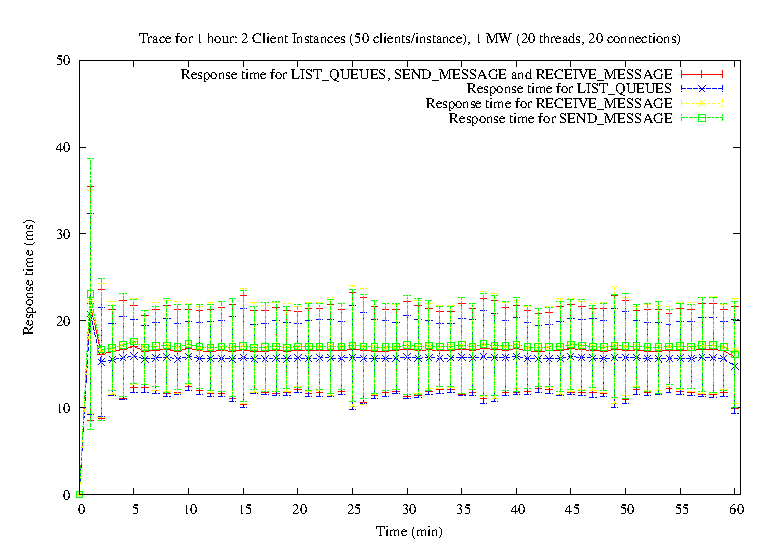
\includegraphics[scale=1.3]{trace1Hour/responseTime/responseTime}
\par\end{centering}

\begin{centering}
\includegraphics[scale=1.28]{trace1Hour/throughput/throughput}
\par\end{centering}

\centering{}\protect\caption{Response time and throughput of an one hour trace with 2 client instances
(50 clients/instance) and 1 middleware instance (20 threads, 20 connections)}
\label{trace}
\end{figure}


The times spent on a specific request:

\begin{tabular}{|c|c|c|}
\hline 
Type of Request & Average Response Time (ms) & Standard Deviation\tabularnewline
\hline 
\hline 
RECEIVE\_MESSAGE & 17.10725 & 5.51819 \tabularnewline
\hline 
SEND\_MESSAGE & 17.1355 & 5.543025\tabularnewline
\hline 
LIST\_QUEUES & 15.7621 & 4.689385\tabularnewline
\hline 
\end{tabular}

The average response time of all types of requests is 16.668.

The time spent on each component during the trace was also calculated
and can be seen in the table below.

\begin{tabular}{|c|c|c|}
\hline 
Time spent on ... & Average Response Time (ms) & Standard Deviation\tabularnewline
\hline 
\hline 
waiting to be picked up by a MW thread & 13.3207 & 4.17608\tabularnewline
\hline 
waiting to get a DB connection & 0.000689706 & 0.216034\tabularnewline
\hline 
executing a DB request & 3.23399 & 2.38918\tabularnewline
\hline 
working inside the MW thread & 3.33539 & 2.51786\tabularnewline
\hline 
\end{tabular}

Based on the values of the above table we would expect that network
time between the client and the middleware and from the middleware
back to the client on average is 16.668 - (13.32 + 3.3539) = WTF??

TIMES TO ENTER: 1.00164, 0.163046 TIMES (NOTHING) INSIDE: 0.0201363,
0.570286 TIMES (DOING) INSIDE: 3.33539, 2.51786

TIMES A SOCKET IS WORKED for a REQUEST TO BE READ: 1, 0

The time to receive a connection is almost non-existant, this is because
we have the same amount of worker threads to connections, so when
a worker thread asks for a connection one can be immediately given
back to the trhead. The time waiting for a worker thread is quite
high and was to be expected since we have 100 clients and only 20
workwer threads. So at any point in time 80 clients connections could
possilby be waiting. Network time is also really low and this makes
sense since the throughput between two instances is (iperf).

As we can see our system is stable under load. In the Figure \ref{trace}
we see that the througput for the RECEIVE\_MESSAGE, SEND\_MESSAGE
and LIST\_QUEUES reqeuests is pretty much the same. This is because
every client issues the exact amount of SEND\_MESSAGE and LIST\_QUEUES
requests and because a RECEIVE\_MESSAGE is only called if a message
is going to be received. The average response time of the LIST\_QUEUES
is a bit lower than the response time of the two other types of requets.
Our assumption was that this is because LIST\_QUEUES does not modify
the database, neither with an INSERT or a DELETE. To verify this claim
we checked the db request average response time for every type of
request shown below:

\begin{tabular}{|c|c|}
\hline 
Type of Request & Average Database Response Time (ms)\tabularnewline
\hline 
\hline 
RECEIVE\_MESSAGE & 3.60231\tabularnewline
\hline 
SEND\_MESSAGE & 3.71801\tabularnewline
\hline 
LIST\_QUEUES & 2.38218\tabularnewline
\hline 
\end{tabular}

Finally we not that in our trace 99.7\% of the requests were served
in less than 50ms, 97\% in under 25ms and 86\% under 20ms.

As was mentioned earlier in this report, we have a \textbf{closed
system}. This means that interactive response time law should apply
to our results. The interactive law states that $R=\frac{N}{X}-Z$
where $R$ is the resonse time, $N$ is the number of clients issuing
requests, $Z$ is the think time and $X$ is the throughput. Our response
time is about 16.668ms, we have 100 clients and our think time is
0, in reality its a positive value since we have to serialize and
deserialize objects but this time is negligible. This means that throughput
should be $X=\frac{N}{R+Z}=\frac{100}{16.668+0}=5.999$. This value
$5.999$ corresponds to the number of requests per ms. Per second
it is $5999$ which is close to the average throughput (of all the
trace) that is $5897$ requests per second. In all the upcoming results
we have verified our results using the interactive law.


\section*{Warm Up and Cool Down}

For all the following experiments, every data point in the plots corresponds
to 10 minute execution of which. From those 10 minutes the first 2
minutes have been removed as the warm up phase and the last 1 minute
as the cool down phase. Those number were derived by checking the
trace and seeing that after 2 minutes our system stabilizes.


\subsection*{Throughput Plots}

In all the following plots the througput was averaged per 20seconds 


\subsection*{Increasing the Message Size}

In this experiment we increased the size of the messages that are
sent between the clients. While running those experiments we realized
clients were receiving the following failed response:

\fbox{\parbox[t]{1\columnwidth}{%
ch.ethz.inf.asl.exceptions.MessagingProtocolException: 

failed to send message ERROR: could not extend file \textquotedbl{}base/16389/16427.6\textquotedbl{}:
No space left on device Hint: Check free disk space. %
}}

After looking around for this problem we realized the problem was
the amount of available memory in our instance's disk. We solved this
problem by increasing the available size of our disks and rerun the
experiments. Afterwards no such failed response was received. The
disk space was increasing because we are not VACUUMing%
\footnote{http://www.postgresql.org/docs/9.3/static/sql-vacuum.html%
} our database and it is known that tuples that are deleted are not
physically removed from their table until a VACUUM is done.

Configuration: The experiment was concuded with:
\begin{itemize}
\item 1 m3.large client instance with 50 clients 
\item 1 m3.large middleware with 20 middleware threads and 20 connections
\item 1 m3.large database
\item message sizes in number of characters that taken were: $1$, $500$,
$1000$, $5000$, $10^{4}$, $2\cdot10^{4}$, $3\cdot10^{4}$, $4\cdot10^{4}$,
$5\cdot10^{4}$, $10^{5}$, $15\cdot10^{4}$, $2\cdot10^{5}$, $5\cdot10^{5}$
and $10^{6}$
\end{itemize}
\textbf{Hypothesis}: We expect to have increased response times as
well as decreased throughput. This is because by increasing the message
size network time needed to send and receive a message will increase
but mostly because the database is going to become slower when handling
more data. 

\begin{figure}[H]


\begin{centering}
\includegraphics[scale=1.2]{increasingMessageSize/throughput/throughput}
\par\end{centering}

\begin{centering}
\includegraphics[scale=1.2]{increasingMessageSize/responseTime/responseTime}
\par\end{centering}

\protect\caption{Increasing the Message Size}
\label{increasingMessageSize}

\end{figure}


As we can see in Figure \ref{increasingMessageSize} there is a huge
increase in the response time as well as a huge decrease in the througput
as expected. We also see that LIST\_QUEUES request have in general
quite high response time but less than both ``SEND\_MESSAGE'' and
``RECEIVE\_MESSAGE''. This was expected but we weren't expecting
such a huge response time for LIST\_QUEUES requests since they do
not move any message around. 

To further investigate why this was the case we checked PostgreSQL
logs were we found this message: ``HINT: Consider increasing the
configuration parameter \textquotedbl{}checkpoint\_segments\textquotedbl{}.
2014-11-05 21:29:32 UTC LOG: checkpoints are occurring too frequently
(2 seconds apart)''. A checkpoint is: ``a point in the transaction
log sequence at which all data files have been updated to reflect
the information in the log. All data files will be flushed to disk.''%
\footnote{http://www.postgresql.org/docs/9.3/static/sql-checkpoint.html%
}. So this could explain why LIST\_QUEUES had such a huge response
time


\subsection*{Increasing the Number of Connections}

\begin{figure}[H]
\begin{centering}
\includegraphics[scale=1.2]{increasingConnections/throughput/throughput}
\par\end{centering}

\begin{centering}
\includegraphics[scale=1.2]{increasingConnections/responseTime/responseTime}
\par\end{centering}

\protect\caption{Increasing the Number of Connections}
\end{figure}



\subsection*{Increasing the Number of Threads}

\begin{figure}[H]
\begin{centering}
\includegraphics[scale=1.2]{increasingThreads/throughput/throughput}
\par\end{centering}

\begin{centering}
\includegraphics[scale=1.2]{increasingThreads/responseTime/responseTime}
\par\end{centering}

\protect\caption{Increasing the Number of Threads}
\end{figure}



\subsection*{Increasing Both Threads and Connections}

\begin{figure}[H]
\begin{centering}
\includegraphics[scale=1.2]{increasingBothClientsAndConnections/throughput/throughput}
\par\end{centering}

\begin{centering}
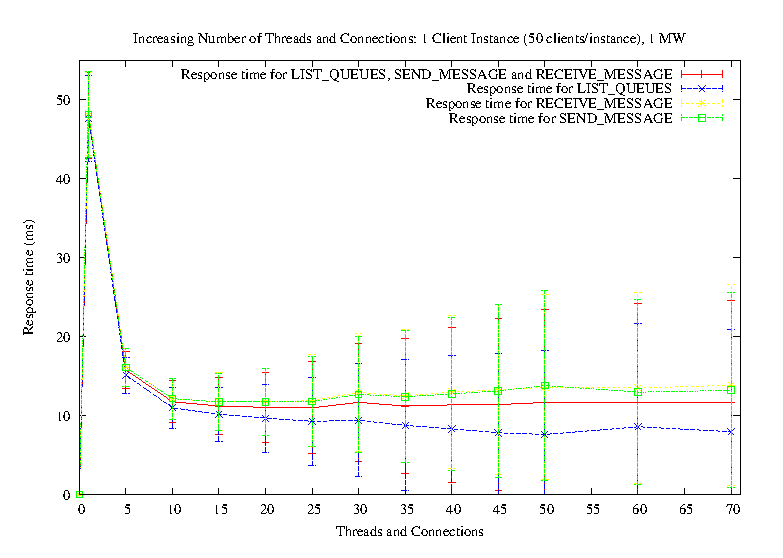
\includegraphics[scale=1.2]{increasingBothClientsAndConnections/responseTime/responseTime}
\par\end{centering}

\centering{}\protect\caption{Increasing Both the Number of Threads and Connections}
\end{figure}



\subsection*{Increasing the Number of Clients}

\begin{figure}[H]
\begin{centering}
\includegraphics[scale=1.2]{increasingClientsOneInstance/throughput/throughput}
\par\end{centering}

\begin{centering}
\includegraphics[scale=1.2]{increasingClientsOneInstance/responseTime/responseTime}\protect\caption{Increasing the Number of Clients}

\par\end{centering}

\end{figure}



\subsection*{Dividing Clients}

Dividing the number of clients 100 ... in the number of instances.
SO initially you have one instance connected to one middleware. Then
you have 2 client instances with 50 clients each connected to 1 middleware.
Then 4 client instances with 25 client each connected to 1 mw each
and finally 10 client instances connected to 1 mw each.

ACtually this experiment was done to show that there is not really
a contention on the client instances.

\begin{figure}[H]


\begin{centering}
\includegraphics[scale=1.2]{dividingClients/responseTime/responseTime}
\par\end{centering}

\begin{centering}
\includegraphics[scale=1.2]{dividingClients/throughput/throughput}
\par\end{centering}

\protect\caption{Breaking Clients into many client instances?}


\end{figure}



\subsection*{Speedup - Finding the bottleneck}

clients and middlewares were m3.large ... Database was r3.2xlarge
to show that the database as the bottleneck ...

Speedup calculated based on response time.

\begin{tabular}{|c|c|c|}
\hline 
Number of Middlewares & Average Response Time for all types of requests (ms) & Standard Deviation\tabularnewline
\hline 
\hline 
1 & 98.3874 & 26.3294\tabularnewline
\hline 
2 & 59.6998 & 20.969\tabularnewline
\hline 
5 & 57.0587 & 21.3355\tabularnewline
\hline 
\end{tabular}

\begin{tabular}{|c|c|c|}
\hline 
Number of Middlewares & Throughput for all types of requests (requests/s) & Standard Deviation\tabularnewline
\hline 
\hline 
1 & 10222.4214286 & 191.01678284\tabularnewline
\hline 
2 & 16906.9833333 & 81.5825047383\tabularnewline
\hline 
5 & 18370.6571429 & 501.37283824\tabularnewline
\hline 
\end{tabular}

\begin{figure}[H]
\begin{centering}
\includegraphics[scale=1.2]{increasingMiddlewares/speedup/throughput}
\par\end{centering}

\begin{centering}
\protect\caption{}

\par\end{centering}

\end{figure}


My next value would be to try with 10 middlewares but this was not
possible because of EC2 limits on having more than 20 instances running
on one availability zone.


\subsection*{Scale Out}

clients and middlewares were m3.large ... Database was r3.2xlarge
to show that the database as the bottleneck ...


\subsection*{Encountered Problems}

During some initial experimenting with the system we had the following
problem, though its seems quite stupid now. We were changing the database
instance type to a better one, from m3.large to m3.2xlarge and the
system's throughput was decreased! It came to our realization that
the new launched database was running the ``us-west-2a'' zone instead
of the ``us-west-2c'', although both were being running in the same
region


\section{Conclusion\label{sec:conclusion}}

At the end the bottleneck is the database.

We believe a great deal of work was done ? (nah) in a nice and consistent
implementation as well as deploying stuff ... 

If we could design the system anew we would not change many aspects
of the system design. What would we do would be to change a bit the
experimental setup so it is easier to run more experiments and get
back graphs instead of manually calling the getResponse and getThroughput
method and passing them to gnuplot by hand. At the end if we could
start the project anew we would have followed a more iterative approach
with fixing something in the system and getting experimental results.
Because the way we followed was build the system, build the experimental
setup and then the experiments and we had to go back to do fixes afterwards
which implied that we had to redo all the expeiments.

At the end we believe we learned a lot about implementing a non-trivial
system and how to benchmark it.
\end{document}
